% Dokumentart und Schrift
\documentclass[11pt, a4paper]{article} % Schriftgröße: 11, Format: A4
\usepackage{cmbright} % Schriftart: CM-Bright

% Eingabe und Sprache
\usepackage[ngerman]{babel} % neue deutsche Rechtschreibung
\usepackage[utf8]{inputenc} % UTF8-Kodierung
\usepackage[T1]{fontenc} % für Umlaute und Akzente

% Seitenränder
\usepackage{geometry}
\geometry{a4paper,left=10mm,right=10mm, top=10mm, bottom=20mm}

% Kopf- und Fußzeile
\usepackage{fancyhdr, lastpage}
\fancyhf{}
\fancyfoot[L]{\textbf{\color{gray3}Echtzeitgrafik Grundlagen SS22}, Aufgabe 1B}
\fancyfoot[R]{\textbf{\color{gray3}Seite \thepage\ von \pageref{LastPage}}}
\fancypagestyle{plain}{}
\pagestyle{fancy}
\renewcommand{\headrulewidth}{0pt}
\renewcommand{\footrulewidth}{1pt}

% Farben: \color{Farbname}TEXT
\usepackage{xcolor} % Farbunterstützung

% Farbdefinitionen
% \definecolor{Name}{Codeart}{Farbcode}  % Beschreibung
\definecolor{beuthcyan}{HTML}{0098A1}	% Türkis der Beuth HS 100%
\definecolor{beuthcyan70}{HTML}{39B7BC}	% Türkis der Beuth HS 70%
\definecolor{beuthcyan30}{HTML}{BEE2E2}	% Türkis der Beuth HS 30%
\definecolor{beuthcyan10}{HTML}{EBF6F6}	% Türkis der Beuth HS 10%
\definecolor{beuthred}{HTML}{EF181E}	% Rot der Beuth HS 10%
\definecolor{gray1}{HTML}{EEEEEE}		% Grauton 1
\definecolor{gray2}{HTML}{CCCCCC}		% Grauton 2
\definecolor{gray3}{HTML}{AAAAAA}		% Grauton 3

% Pakete für mathematische Dokumente
\usepackage{mathastext} % mathematische Formeln nicht kursiv schreiben
\usepackage{amsmath,amsfonts,amssymb,stmaryrd}
\usepackage{multicol}
\usepackage{colortbl}

% Bilder
\usepackage{graphicx}

% Pakete für Zeichnungen und Graphenverläufe
\usepackage{pgfplots}
\usepackage{tikz}
\usepackage{tkz-euclide}

% Paket für Polynome
\usepackage{polynom}

% -----------------------------------------------------------------

\begin{document}
	\section*{Echtzeitgrafik Grundlagen SS22, Aufgabe 1B}
	\textbf{BHT Berlin, Medieninformatik Bachelor, 4. Semester} \\
	\textbf{Dozent:} A. Schwarz \\
	\textbf{Name:} \textbf{\color{gray3}Florian Kate}, \textbf{Matrikelnummer:} 923081 \\
	\textbf{Datum:} 29.04.2022

\subsection*{1B.1 Transformation}
Geben ist ein Dreieck mit den drei Punkten $A(0,1)$, $B(0,-1)$ und $C(2,-1)$. Führen sie im Folgenden die drei Transformationen nacheinander aus. Zuerst die Translation, anschließend rotieren sie das verschobene Dreieck und zum Schluss skalieren sie das verschobene und rotierte Dreieck. Zeichnen sie die jeweiligen Zwischenergebnisse in das leere Koordinatensystem und notieren sie
die jeweils geforderten Antwort. Also die jeweilige 4x4 Matrix und das Zwischenergebnis der Transformationskette.
\begin{figure}[h]
	\begin{tikzpicture}
		\tkzInit[xmax=6,ymax=6,xmin=-6,ymin=-6]
		\tkzGrid[line width=0.1mm, color=gray]
		\tkzAxeXY
		\coordinate[label=$A$](A) at (0,1);
		\coordinate[label=$B$](B) at (0,-1);
		\coordinate[label=$C$](C) at (2,-1);
		\fill[black] (A) circle(2pt);
		\fill[black] (B) circle(2pt);
		\fill[black] (C) circle(2pt);
		\draw[line width=0.3mm] (A) -- (B) -- (C) -- (A);
		\draw[fill=beuthred, opacity=0.5] (A) -- (B) -- (C) -- (A);
	\end{tikzpicture}
\end{figure}

\newpage
\subsubsection*{1. Translation}
Führen Sie eine Translation mit den drei Punkten aus. Die Punkte sollen nach der Translation die Koordinaten $A(4,2)$, $B(4,0)$ und $C(6,0)$ haben. Notieren Sie die entsprechende Translationsmatrix und zeichnen Sie den Translationsvektor ein. \\[0.1cm]
Translationsmatrix: $\begin{bmatrix}
	P'_x \\ P'_y \\ P'_z \\ 1
\end{bmatrix} = \begin{bmatrix}
P_x + T_x \\ P_y + T_y \\ P_z + T_z \\ 1
\end{bmatrix} = \begin{bmatrix}
1 & 0 & 0 & T_x \\ 0 & 1 & 0 & T_y \\ 0 & 0 & 1 & T_z \\ 0 & 0 & 0 & 1
\end{bmatrix} \begin{bmatrix}
P_x \\ P_y \\ P_z \\ 1
\end{bmatrix}$ \\
Punkt A: $\begin{bmatrix}
	4 \\ 2 \\ 0 \\ 1
\end{bmatrix} = \begin{bmatrix}
	0+(4-0) \\ -1+(2-1) \\ 0+0 \\ 1
\end{bmatrix} = \begin{bmatrix}
	1 & 0 & 0 & 4 \\ 0 & 1 & 0 & 1 \\ 0 & 0 & 1 & 0 \\ 0 & 0 & 0 & 1
\end{bmatrix} \begin{bmatrix}
	0 \\ 1 \\ 0 \\ 1
\end{bmatrix}$ \\
Punkt B: $\begin{bmatrix}
	4 \\ 0 \\ 0 \\ 1
\end{bmatrix} = \begin{bmatrix}
	0+(4-0) \\ -1+(0-(-1)) \\ 0+0 \\ 1
\end{bmatrix} = \begin{bmatrix}
	1 & 0 & 0 & 4 \\ 0 & 1 & 0 & 1 \\ 0 & 0 & 1 & 0 \\ 0 & 0 & 0 & 1
\end{bmatrix} \begin{bmatrix}
	0 \\ -1 \\ 0 \\ 1
\end{bmatrix}$ \\
Punkt C: $\begin{bmatrix}
	6 \\ 0 \\ 0 \\ 1
\end{bmatrix} = \begin{bmatrix}
	2+(4-0) \\ -1+(0-(-1)) \\ 0+0 \\ 1
\end{bmatrix} = \begin{bmatrix}
	1 & 0 & 0 & 4 \\ 0 & 1 & 0 & 1 \\ 0 & 0 & 1 & 0 \\ 0 & 0 & 0 & 1
\end{bmatrix} \begin{bmatrix}
	2 \\ -1 \\ 0 \\ 1
\end{bmatrix}$ \\
Translationvektor T: $\begin{bmatrix}
	T_x \\ T_y \\ T_z \\ 1
\end{bmatrix} = \begin{bmatrix}
	4 \\ 1 \\ 0 \\ 1
\end{bmatrix}$ \\[0.5cm]
\begin{figure}[h]
	\begin{tikzpicture}
		\tkzInit[xmax=6,ymax=6,xmin=-6,ymin=-6]
		\tkzGrid[line width=0.1mm, color=gray]
		\tkzAxeXY
		\coordinate[label=$A$](A) at (4,2);
		\coordinate[label=$B$](B) at (4,0);
		\coordinate[label=$C$](C) at (6,0);
		\fill[black] (A) circle(2pt);
		\fill[black] (B) circle(2pt);
		\fill[black] (C) circle(2pt);
		\draw[line width=0.3mm] (A) -- (B) -- (C) -- (A);
		\draw[fill=beuthred, opacity=0.5] (A) -- (B) -- (C) -- (A);
		\draw[line width=0.5mm, color=beuthred, ->] (0,0) -- (4,1) node[pos=0.5, above]{$T$};
	\end{tikzpicture}
\end{figure}

\newpage
\subsubsection*{2. Rotation}
Rotieren sie das verschobene Dreieck um $\alpha=45^\circ$ um den Koordinatenursprung. Notieren sie die entsprechende Rotationsmatrix. Zeichnen sie die Lösung ein und notieren sie das Zwischenergebnis der Transformationskette. \\[0.1cm]
\textbf{Anmerkung:} Wir rotieren hier um die Z-Achse. \\
Rotationsmatrix $R_z$: $\begin{bmatrix}
	P''_x \\ P''_y \\ P''_z \\ 1
\end{bmatrix} = \begin{bmatrix}
	\cos(\alpha) & -\sin(\alpha) & 0 & 0 \\ \sin(\alpha) & \cos(\alpha) & 0 & 0 \\ 0 & 0 & 1 & 0 \\ 0 & 0 & 0 & 1
\end{bmatrix} \begin{bmatrix}
	P'_x \\ P'_y \\ P'_z \\ 1
\end{bmatrix}$ \\
Zwischenergebnis der Transformationskette: $\begin{bmatrix}
	P''_x \\ P''_y \\ P''_z \\ 1
\end{bmatrix} = \begin{bmatrix}
	\cos(45^\circ) & -\sin(45^\circ) & 0 & 0 \\ \sin(45^\circ) & \cos(45^\circ) & 0 & 0 \\ 0 & 0 & 1 & 0 \\ 0 & 0 & 0 & 1
\end{bmatrix} \begin{bmatrix}
1 & 0 & 0 & 4 \\ 0 & 1 & 0 & 1 \\ 0 & 0 & 1 & 0 \\ 0 & 0 & 0 & 1
\end{bmatrix} \begin{bmatrix}
	P_x \\ P_y \\ P_z \\ 1
\end{bmatrix}$ \\
Punkt A: $\begin{bmatrix}
	P''_x \\ P''_y \\ P''_z \\ 1
\end{bmatrix} = \begin{bmatrix}
	\cos(45^\circ) & -\sin(45^\circ) & 0 & 0 \\ \sin(45^\circ) & \cos(45^\circ) & 0 & 0 \\ 0 & 0 & 1 & 0 \\ 0 & 0 & 0 & 1
\end{bmatrix} \begin{bmatrix}
	4 \\ 2 \\ 0 \\ 1
\end{bmatrix} = \begin{bmatrix}
1,41 \\ 4,24 \\ 0 \\ 1
\end{bmatrix}$ \\
Punkt B: $\begin{bmatrix}
	P''_x \\ P''_y \\ P''_z \\ 1
\end{bmatrix} = \begin{bmatrix}
	\cos(45^\circ) & -\sin(45^\circ) & 0 & 0 \\ \sin(45^\circ) & \cos(45^\circ) & 0 & 0 \\ 0 & 0 & 1 & 0 \\ 0 & 0 & 0 & 1
\end{bmatrix} \begin{bmatrix}
	4 \\ 0 \\ 0 \\ 1
\end{bmatrix} = \begin{bmatrix}
2,83 \\ 2,83 \\ 0 \\ 1
\end{bmatrix}$ \\
Punkt C: $\begin{bmatrix}
	P''_x \\ P''_y \\ P''_z \\ 1
\end{bmatrix} = \begin{bmatrix}
	\cos(45^\circ) & -\sin(45^\circ) & 0 & 0 \\ \sin(45^\circ) & \cos(45^\circ) & 0 & 0 \\ 0 & 0 & 1 & 0 \\ 0 & 0 & 0 & 1
\end{bmatrix} \begin{bmatrix}
	6 \\ 0 \\ 0 \\ 1
\end{bmatrix} = \begin{bmatrix}
4,24 \\ 4,24 \\ 0 \\ 1
\end{bmatrix}$ \\[0.5cm]
\begin{figure}[h]
	\begin{tikzpicture}
		\tkzInit[xmax=6,ymax=6,xmin=-6,ymin=-6]
		\tkzGrid[line width=0.1mm, color=gray]
		\tkzAxeXY
		\coordinate[label=$A$](A) at (1.41,4.24);
		\coordinate[label=$B$](B) at (2.83,2.83);
		\coordinate[label=$C$](C) at (4.24,4.24);
		\fill[black] (A) circle(2pt);
		\fill[black] (B) circle(2pt);
		\fill[black] (C) circle(2pt);
		\draw[line width=0.3mm] (A) -- (B) -- (C) -- (A);
		\draw[fill=beuthred, opacity=0.5] (A) -- (B) -- (C) -- (A);
	\end{tikzpicture}
\end{figure}

\newpage
\subsubsection*{3. Skalierung}
Skalieren sie das verschobene und rotierte Dreieck mit dem Vektor (2,1). Notieren sie die entsprechende Skalierungsmatrix, Endergebnis der Transformationskette. \\[0.1cm]
Skalierungsmatrix: $\begin{bmatrix}
	P'''_x \\ P'''_y \\ P'''_z \\ 1
\end{bmatrix} = \begin{bmatrix}
	S_x & 0 & 0 & 0 \\ 0 & S_y & 0 & 0 \\ 0 & 0 & S_z & 0 \\ 0 & 0 & 0 & 1
\end{bmatrix} \begin{bmatrix}
	P''_x \\ P''_y \\ P''_z \\ 1
\end{bmatrix}$ \\
Endergebnis der Transformationskette: $\begin{bmatrix}
	P'''_x \\ P'''_y \\ P'''_z \\ 1
\end{bmatrix} = \begin{bmatrix}
2 & 0 & 0 & 0 \\ 0 & 1 & 0 & 0 \\ 0 & 0 & 0 & 0 \\ 0 & 0 & 0 & 1
\end{bmatrix} \begin{bmatrix}
	\cos(45^\circ) & -\sin(45^\circ) & 0 & 0 \\ \sin(45^\circ) & \cos(45^\circ) & 0 & 0 \\ 0 & 0 & 1 & 0 \\ 0 & 0 & 0 & 1
\end{bmatrix} \begin{bmatrix}
	1 & 0 & 0 & 4 \\ 0 & 1 & 0 & 1 \\ 0 & 0 & 1 & 0 \\ 0 & 0 & 0 & 1
\end{bmatrix} \begin{bmatrix}
	P_x \\ P_y \\ P_z \\ 1
\end{bmatrix}$ \\
Punkt A: $\begin{bmatrix}
	P'''_x \\ P'''_y \\ P'''_z \\ 1
\end{bmatrix} = \begin{bmatrix}
	2 & 0 & 0 & 0 \\ 0 & 1 & 0 & 0 \\ 0 & 0 & 0 & 0 \\ 0 & 0 & 0 & 1
\end{bmatrix} \begin{bmatrix}
	1,41 \\ 4,24 \\ 0 \\ 1
\end{bmatrix} = \begin{bmatrix}
2.83 \\ 4,24 \\ 0 \\ 1
\end{bmatrix}$ \\
Punkt B: $\begin{bmatrix}
	P'''_x \\ P'''_y \\ P'''_z \\ 1
\end{bmatrix} = \begin{bmatrix}
	2 & 0 & 0 & 0 \\ 0 & 1 & 0 & 0 \\ 0 & 0 & 0 & 0 \\ 0 & 0 & 0 & 1
\end{bmatrix} \begin{bmatrix}
	2,83 \\ 2,83 \\ 0 \\ 1
\end{bmatrix} = \begin{bmatrix}
	5,65 \\ 2,83 \\ 0 \\ 1
\end{bmatrix}$ \\
Punkt C: $\begin{bmatrix}
	P'''_x \\ P'''_y \\ P'''_z \\ 1
\end{bmatrix} = \begin{bmatrix}
	2 & 0 & 0 & 0 \\ 0 & 1 & 0 & 0 \\ 0 & 0 & 0 & 0 \\ 0 & 0 & 0 & 1
\end{bmatrix} \begin{bmatrix}
	4,24 \\ 4,24 \\ 0 \\ 1
\end{bmatrix} = \begin{bmatrix}
	8,49 \\ 4,24 \\ 0 \\ 1
\end{bmatrix}$ \\
\begin{figure}[h]
	\begin{tikzpicture}
		\tkzInit[xmax=9,ymax=6,xmin=-6,ymin=-6]
		\tkzGrid[line width=0.1mm, color=gray]
		\tkzAxeXY
		\coordinate[label=$A$](A) at (2.83,4.24);
		\coordinate[label=$B$](B) at (5.65,2.83);
		\coordinate[label=$C$](C) at (8.49,4.24);
		\fill[black] (A) circle(2pt);
		\fill[black] (B) circle(2pt);
		\fill[black] (C) circle(2pt);
		\draw[line width=0.3mm] (A) -- (B) -- (C) -- (A);
		\draw[fill=beuthred, opacity=0.5] (A) -- (B) -- (C) -- (A);
	\end{tikzpicture}
\end{figure}

\newpage
\subsubsection*{Umgekehrte Reihenfolge}
Führen sie die Transformation des \textbf{ursprünglichen Dreieckes} noch mal in umgekehrter Reihenfolge aus. Also beginnen sie mit der Skalierung, rotieren sie dann das skalierte Dreieck und anschließend führen sie die Translation aus. Zeichnen sie das endgültige Ergebnis in das Koordinatensystem ein und notieren sie die endgültige Transformationsmatrix. Beschreiben sie kurz (1-2 Sätze oder Stichpunkte) wie sich die beiden Ergebnisse unterscheiden. \\[0.1cm]
Transformationsmatrix: $\begin{bmatrix}
	P'_x \\ P'_y \\ P'_z \\ 1
\end{bmatrix} = \begin{bmatrix}
	1 & 0 & 0 & 4 \\ 0 & 1 & 0 & 1 \\ 0 & 0 & 1 & 0 \\ 0 & 0 & 0 & 1
\end{bmatrix} \begin{bmatrix}
\cos(45^\circ) & -\sin(45^\circ) & 0 & 0 \\ \sin(45^\circ) & \cos(45^\circ) & 0 & 0 \\ 0 & 0 & 1 & 0 \\ 0 & 0 & 0 & 1
\end{bmatrix} \begin{bmatrix}
2 & 0 & 0 & 0 \\ 0 & 1 & 0 & 0 \\ 0 & 0 & 0 & 0 \\ 0 & 0 & 0 & 1
\end{bmatrix} \begin{bmatrix}
P_x \\ P_y \\ P_z \\ 1
\end{bmatrix}$ \\
Punkt A: $\begin{bmatrix}
	P'_x \\ P'_y \\ P'_z \\ 1
\end{bmatrix} = \begin{bmatrix}
	1 & 0 & 0 & 4 \\ 0 & 1 & 0 & 1 \\ 0 & 0 & 1 & 0 \\ 0 & 0 & 0 & 1
\end{bmatrix} \begin{bmatrix}
	\cos(45^\circ) & -\sin(45^\circ) & 0 & 0 \\ \sin(45^\circ) & \cos(45^\circ) & 0 & 0 \\ 0 & 0 & 1 & 0 \\ 0 & 0 & 0 & 1
\end{bmatrix} \begin{bmatrix}
	2 & 0 & 0 & 0 \\ 0 & 1 & 0 & 0 \\ 0 & 0 & 0 & 0 \\ 0 & 0 & 0 & 1
\end{bmatrix} \begin{bmatrix}
	0 \\ 1 \\ 0 \\ 1
\end{bmatrix} = \begin{bmatrix}
3.29 \\ 1.71 \\ 0 \\ 1
\end{bmatrix}$ \\
Punkt B: $\begin{bmatrix}
	P'_x \\ P'_y \\ P'_z \\ 1
\end{bmatrix} = \begin{bmatrix}
	1 & 0 & 0 & 4 \\ 0 & 1 & 0 & 1 \\ 0 & 0 & 1 & 0 \\ 0 & 0 & 0 & 1
\end{bmatrix} \begin{bmatrix}
	\cos(45^\circ) & -\sin(45^\circ) & 0 & 0 \\ \sin(45^\circ) & \cos(45^\circ) & 0 & 0 \\ 0 & 0 & 1 & 0 \\ 0 & 0 & 0 & 1
\end{bmatrix} \begin{bmatrix}
	2 & 0 & 0 & 0 \\ 0 & 1 & 0 & 0 \\ 0 & 0 & 0 & 0 \\ 0 & 0 & 0 & 1
\end{bmatrix} \begin{bmatrix}
	0 \\ -1 \\ 0 \\ 1
\end{bmatrix} = \begin{bmatrix}
	4.71 \\ 0.29 \\ 0 \\ 1
\end{bmatrix}$ \\
Punkt C: $\begin{bmatrix}
	P'_x \\ P'_y \\ P'_z \\ 1
\end{bmatrix} = \begin{bmatrix}
	1 & 0 & 0 & 4 \\ 0 & 1 & 0 & 1 \\ 0 & 0 & 1 & 0 \\ 0 & 0 & 0 & 1
\end{bmatrix} \begin{bmatrix}
	\cos(45^\circ) & -\sin(45^\circ) & 0 & 0 \\ \sin(45^\circ) & \cos(45^\circ) & 0 & 0 \\ 0 & 0 & 1 & 0 \\ 0 & 0 & 0 & 1
\end{bmatrix} \begin{bmatrix}
	2 & 0 & 0 & 0 \\ 0 & 1 & 0 & 0 \\ 0 & 0 & 0 & 0 \\ 0 & 0 & 0 & 1
\end{bmatrix} \begin{bmatrix}
	2 \\ -1 \\ 0 \\ 1
\end{bmatrix} = \begin{bmatrix}
	7.54 \\ 3.12 \\ 0 \\ 1
\end{bmatrix}$ \\
\begin{figure}[h]
	\begin{tikzpicture}
		\tkzInit[xmax=9,ymax=6,xmin=-6,ymin=-6]
		\tkzGrid[line width=0.1mm, color=gray]
		\tkzAxeXY
		\coordinate[label=$A$](A) at (3.29,1.71);
		\coordinate[label=$B$](B) at (4.71,0.29);
		\coordinate[label=$C$](C) at (7.54,3.12);
		\fill[black] (A) circle(2pt);
		\fill[black] (B) circle(2pt);
		\fill[black] (C) circle(2pt);
		\draw[line width=0.3mm] (A) -- (B) -- (C) -- (A);
		\draw[fill=beuthred, opacity=0.5] (A) -- (B) -- (C) -- (A);
	\end{tikzpicture}
\end{figure} \\
Die Dreiecke sehen grundverschieden aus, da wir erst verschoben, dann rotiert (weiter entfernt zum Ursprung) und danach skaliert haben. In umgekehrter Reihenfolge haben wir erst skaliert, dann rotiert (nahe dem Ursprung) und zuletzt verschoben. Dadurch ist das zweite Dreieck auch \textit{"weiter unten"} auf der y-Achse, obwohl in einem ähnlichen Bereich auf der x-Achse.

\newpage
\subsubsection*{Lokale Rotation}
Beschreiben die kurz die theoretischen Transformationsschritt die gegangen werden müssen, um folgendes Ergebnis erhalten. \\[0.1cm]
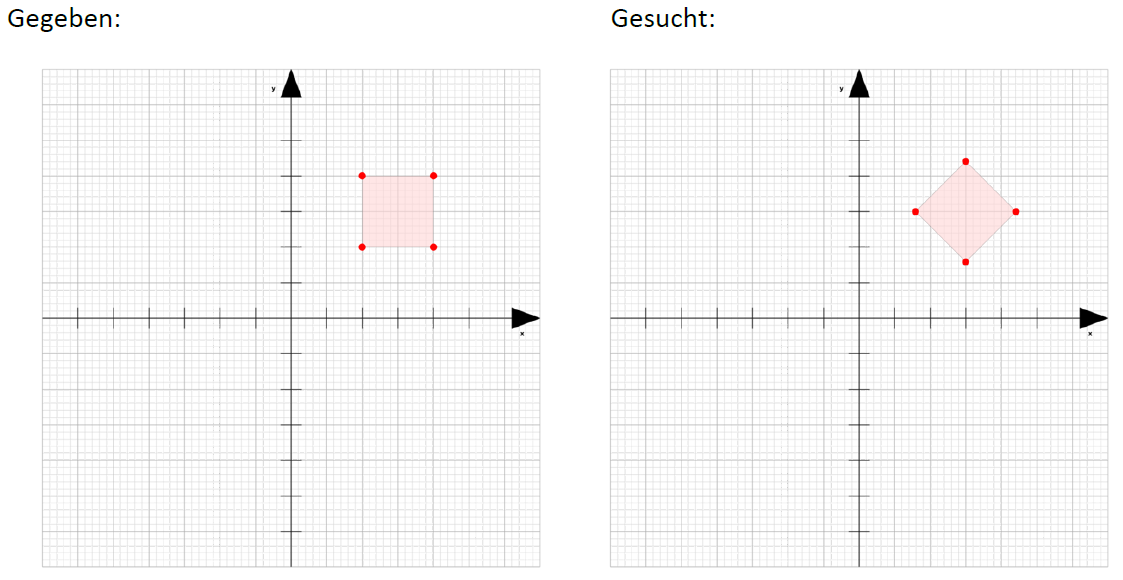
\includegraphics[scale=0.5]{lr.png} \\[0.1cm]
Wir suchen zuerst den Mittelpunkt des Quadrats: $M(3,3)$. Danach verschieben wir alle Punkte des Quadrats, sodass der Mittelpunkt nun im Koordinatenursprung liegt. Dann rotieren wir um $45^\circ$ und verschieben anschließend alle Punkte wieder zurück. \\
Transformationsmatrix: $\begin{bmatrix}
	P'_x \\ P'_y \\ P'_z \\ 1
\end{bmatrix} = \begin{bmatrix}
	1 & 0 & 0 & 3 \\ 0 & 1 & 0 & 3 \\ 0 & 0 & 1 & 0 \\ 0 & 0 & 0 & 1
\end{bmatrix} \begin{bmatrix}
	\cos(45^\circ) & -\sin(45^\circ) & 0 & 0 \\ \sin(45^\circ) & \cos(45^\circ) & 0 & 0 \\ 0 & 0 & 1 & 0 \\ 0 & 0 & 0 & 1
\end{bmatrix} \begin{bmatrix}
1 & 0 & 0 & -3 \\ 0 & 1 & 0 & -3 \\ 0 & 0 & 1 & 0 \\ 0 & 0 & 0 & 1
\end{bmatrix} \begin{bmatrix}
	P_x \\ P_y \\ P_z \\ 1
\end{bmatrix}$

\subsection*{1B.2 Szenegraph}
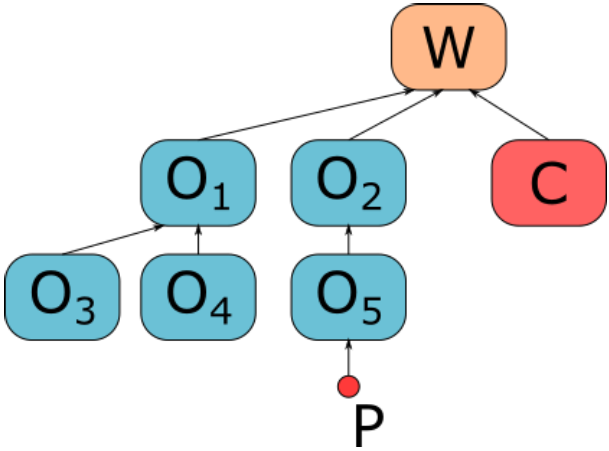
\includegraphics[scale=0.5]{sg.png} \\
Gegeben ist eine Szene mit 5 Objekten und einer Kamera, die Objekte sind hierarchisch geordnet und bilden folgenden Szenengraph. In dieser Aufgabe betrachten wir den Punkt P, dieser ist ein Kindelement bzw. ein Bestandteil des Objektes $O_5$. Der Punkt hat in dem lokalen Koordinatensystem des Objektes $O_5$ die Koordinaten P [1,1,0]. Das Objekt $O_5$ wird wie folgt transformiert: Zuerst wird das Objekt um den Vektor $\vec{s}$ [2,3,1] skaliert ($S_1$) und anschließend um die z-Achse um $90^\circ$ rotiert ($R_1$). Das Objekt $O_5$ ist wiederum ein Kindelement von Objekt $O_2$. $O_2$ wird wiederum wie folgt transformiert: zuerst wird das Objekt um $90^\circ$ um die y-Achse gedreht ($R_2$). Anschließend wird das Objekt mit den Skalierungsvektor $\vec{s}$ [1, 0.5, 1] skaliert ($S_2$). Zuletzt wird das Objekt um den Vektor $\vec{t}$ [1,0,-3] verschoben ($T_1$). \\
Punkt P in Weltkoordinaten $P'= T_1S_2R_2R_1S_1\cdot P$ \\[0.5cm]
$P' = \underbrace{\begin{bmatrix}
	1 & 0 & 0 & 1 \\ 0 & 1 & 0 & 0 \\ 0 & 0 & 1 & -3 \\ 0 & 0 & 0 & 1
\end{bmatrix}}_{T_1} \underbrace{\begin{bmatrix}
1 & 0 & 0 & 0 \\ 0 & 0,5 & 0 & 0 \\ 0 & 0 & 1 & 0 \\ 0 & 0 & 0 & 1
\end{bmatrix}}_{S_2} \underbrace{\begin{bmatrix}
\cos(90^\circ) & 0 & \sin(90^\circ) & 0 \\ 0 & 1 & 0 & 0 \\ -\sin(90^\circ) & 0 & \cos(90^\circ) & 0 \\ 0 & 0 & 0 & 1
\end{bmatrix}}_{R_2} \cdot$ \\
$\underbrace{\begin{bmatrix}
\cos(90^\circ) & -\sin(90^\circ) & 0 & 0 \\ \sin(90^\circ) & \cos(90^\circ) & 0 & 0 \\ 0 & 0 & 1 & 0 \\ 0 & 0 & 0 & 1
\end{bmatrix}}_{R_1} \underbrace{\begin{bmatrix}
2 & 0 & 0 & 0 \\ 0 & 3 & 0 & 0 \\ 0 & 0 & 1 & 0 \\ 0 & 0 & 0 & 1
\end{bmatrix}}_{S_1} \underbrace{\begin{bmatrix}
1 \\ 1 \\ 0 \\ 1
\end{bmatrix}}_{P} = \begin{bmatrix}
1 \\ 1 \\ 0 \\ 1
\end{bmatrix}$ \\
Modelmatrix $M = T_1S_2R_2R_1S_1 = \underbrace{\begin{bmatrix}
		1 & 0 & 0 & 1 \\ 0 & 1 & 0 & 0 \\ 0 & 0 & 1 & -3 \\ 0 & 0 & 0 & 1
\end{bmatrix}}_{T_1} \underbrace{\begin{bmatrix}
		1 & 0 & 0 & 0 \\ 0 & 0,5 & 0 & 0 \\ 0 & 0 & 1 & 0 \\ 0 & 0 & 0 & 1
\end{bmatrix}}_{S_2} \underbrace{\begin{bmatrix}
		\cos(90^\circ) & 0 & \sin(90^\circ) & 0 \\ 0 & 1 & 0 & 0 \\ -\sin(90^\circ) & 0 & \cos(90^\circ) & 0 \\ 0 & 0 & 0 & 1
\end{bmatrix}}_{R_2} \cdot$ \\
$\underbrace{\begin{bmatrix}
		\cos(90^\circ) & -\sin(90^\circ) & 0 & 0 \\ \sin(90^\circ) & \cos(90^\circ) & 0 & 0 \\ 0 & 0 & 1 & 0 \\ 0 & 0 & 0 & 1
\end{bmatrix}}_{R_1} \underbrace{\begin{bmatrix}
		2 & 0 & 0 & 0 \\ 0 & 3 & 0 & 0 \\ 0 & 0 & 1 & 0 \\ 0 & 0 & 0 & 1
\end{bmatrix}}_{S_1} = \begin{bmatrix}
0 & 0 & 1 & 1 \\ 1 & 0 & 0 & 0 \\ 0 & 3 & 0 & -3 \\ 0 & 0 & 0 & 1
\end{bmatrix}$ \\[1.0cm]
%
\textbf{Anmerkung:} Aufgrund der Komplexität der Berechnungen und der hohen Fehleranfälligkeit bei Berechnungen per Hand mit dem Falk-Schema habe ich die Ergebnisse mit Octave berechnet.

\end{document}